\documentclass[main.tex]{subfiles}

\begin{document}
%-------------------------------------------------------------------------------
%---------------------------------- Section 1 ----------------------------------
%-------------------------------------------------------------------------------
\section{Vektoranalízis}

%-------------------------------------------------------------------------------
%-------------------------------- Subsection 1.1 -------------------------------
%-------------------------------------------------------------------------------
\subsection{Ismétlés}

\defi{0}{0}{Vektortér}

Legyen $V$ egy nemüreshalmaz és $+$, $\circ$ két művelet,
$\mathbb{T}$ számtest $\left( V; +; \circ \right)$ $\mathbb{T}$
test feletti vektortér (lineáris tér), ha teljesülnek az alábbi
feltételek:
\begin{itemize}
  \item $\left( V ; + \right)$ Abel-csoport,

  \item ha $\forall \, \alpha; \beta \in \mathbb{T}$
        és $\rvec{x} \in V$,
        akkor $(\alpha \circ \beta) \circ \rvec{x}
          = \alpha \circ (\beta \circ \rvec{x})$,

  \item ha $\varepsilon \in \mathbb{T}$ egységelem,
        akkor $\forall \, \rvec{x} \in V$ esetén
        $\varepsilon \circ \rvec{x}
          = \rvec{x} \circ \varepsilon
          = \rvec{x}$,

  \item ha $\forall \, \alpha; \beta \in \mathbb{T}$
        és $\rvec{x}; \rvec{y} \in V$, akkor
        $(\alpha + \beta) \circ \rvec{x}
          = \alpha \circ \rvec{x} + \beta \circ \rvec{x}$
        és $\alpha \circ (\rvec{x} + \rvec{y})
          = \alpha \circ \rvec{x} + \alpha \circ \rvec{y}$.
\end{itemize}



\defi{1}{.33}{Lineáris leképezés}

Legyenek $V_1$ és $V_2$ ugyanazon test ($\mathbb{R}$ vagy $\mathbb{C}$)
feletti vektorterek. Legyen $\varphi: V_1 \rightarrow V_2$ leképezés,
melyet lineáris leképezésnek nevezünk, ha
\begin{gather*}
  \varphi ( \alpha \rvec{a} + \beta \rvec{b} )
  = \alpha \cdot \varphi ( \rvec{a} )
  + \beta \cdot \varphi ( \rvec{b} )
\end{gather*}
bármely $\rvec{a} ; \rvec{b} \in V_1$ és
$\alpha; \beta \in \mathbb{R}$ esetén teljesül.



\defi{1}{.33}{Homomorfizmus}
\begin{gather*}
  \Hom ( V_1; V_2 ) := \left\{
  \varphi : V_1 \rightarrow V_2 \; | \; \varphi \; \text{lineáris}
  \right\}
\end{gather*}



\defi{1}{.33}{Endomorfizmus}
\begin{gather*}
  V_1 = V_2 = V \; \rightarrow \;
  \Hom ( V; V ) = \End (V)
\end{gather*}



\megj{1}{.33}{Lineáris leképezések mátrixreprezentációja}

Legyen $V_1$ és $V_2$ ugyanazon test feletti vektorterek,
$\dim(V_1) = n$ és $\dim(V_2) = k$. Ekkor a $\varphi: V_1 \rightarrow V_2$
leképezést reprezentáló mátrix $n \cross k$ dimenziós.

\vspace{.5em}
$\left( \Hom(V_1; V_2); +; \lambda\right)$ és
$\left( \mathcal{M}_{k \cross n}; +; \lambda\right)$
vektorterek izomorfok egymással.



\defi{1}{.33}{Skaláris szorzás}

Legyen adva egy $\mathbb{R}$ feletti vektortér,
és értelmezzük a $< \, ; \, > \, : V \cross V \rightarrow \mathbb{R}$
függvényt, melyet skaláris szorzatnak mondunk,
ha teljesíti az alábbiakat:
\begin{itemize}
  \item szimmetrikus
        \tabto{3cm} – \tabto{3.6cm}
        $\scalar{\rvec{x}}{\rvec{y}}
          \;=\;
          \scalar{\rvec{y}}{\rvec{x}}$
        \tabto{12cm}
        $\forall \, \rvec{x}; \rvec{y} \in V$

  \item homogén
        \tabto{3cm} – \tabto{3.6cm}
        $\scalar{\alpha \, \rvec{x}}{\rvec{y}}
          \;=\;
          \alpha \scalar{\rvec{x}}{\rvec{y}}$
        \tabto{12cm}
        $\forall \, \rvec{x}; \rvec{y} \in V$,
        $\forall \, \alpha \in \mathbb{R}$

  \item additív
        \tabto{3cm} – \tabto{3.6cm}
        $\scalar{\rvec{x}_1 + \rvec{x}_2}{\rvec{y}}
          \;=\;
          \scalar{\rvec{x}_1}{\rvec{y}} + \scalar{\rvec{x}_2}{\rvec{y}}$
        \tabto{12cm}
        $\forall \, \rvec{x}_1; \rvec{x}_2; \rvec{y} \in V$

  \item nemnegatív
        \tabto{3cm} – \tabto{3.6cm}
        $\scalar{\rvec{x}}{\rvec{x}} \; \geqq \; 0$
        \tabto{12cm}
        egyenlőség $\Leftrightarrow \rvec{x} = \rvec{0}$
\end{itemize}


\megj{1}{.33}

A skaláris szorzás szimmetrikus billineáris forma,
amely az Euklideszi térben értelmezve van.


%-------------------------------------------------------------------------------
%-------------------------------- Subsection 1.2 -------------------------------
%-------------------------------------------------------------------------------
\subsection{Alapfogalmak}


\defi{1}{.33}{Konvektor}

Legyen $V$ egy $\mathbb{R}$ feletti vektortér.
$V^{*} := \Hom(V; \mathbb{R})$ elemeit
($\alpha: V \rightarrow \mathbb{R}$)
lineáris funkcionáloknak, lineáris
formáknak, vagy 1-formáknak nevezzük.
Mivel $\alpha$ lineáris leképezés, ezért
\begin{gather*}
  \alpha(a \rvec{v} + b \rvec{w})
  = a \, \alpha(\rvec{v}) + b \, \alpha(\rvec{w})
  \text{ teljesül.}
\end{gather*}



\allit{1}{.33}{Duális tér}

Legyen $\alpha; \beta \in V^{*}$, $\rvec{v} \in V$,
$a \in \mathbb{R}$. A fenti módon teljesülnek az alábbiak:
\begin{gather*}
  (\alpha + \beta)(\rvec{v}) := \alpha(\rvec{w}) + \beta(\rvec{w}),
  \hspace{20mm}
  (a \, \alpha)(\rvec{w}) := a \, \alpha(\rvec{w}).
\end{gather*}

Ekkor $V^{*}$ vektortérré tehető,
$V$ vektortér duális terének nevezzük.



\jel{1}{0}{Bázis}
\begin{itemize}
  \item ${\left\{
              \uvec{e}_1 \; ; \;
              \uvec{e}_2 \; ; \;
              \dots \; ; \;
              \uvec{e}_n
              \right\}}$
        \tabto{4cm} –  \tabto{4.6cm}
        ortonormált / standard bázis

  \item ${\left\{
              \rvec{b}_1 \; ; \;
              \rvec{b}_2 \; ; \;
              \dots \; ; \;
              \rvec{b}_n
              \right\}}$
        \tabto{4cm} –  \tabto{4.6cm}
        tetszőleges bázis
\end{itemize}

$!\exists \left(
  r^1 \; ; \;
  r^2 \; ; \;
  \dots \; ; \;
  r^n
  \right)$,
melyre teljesül, hogy
\begin{gather*}
  \rvec{v}
  = r^1 \rvec{b}_1
  + r^2 \rvec{b}_2
  + \dots
  + r^n \rvec{b}_n
  = \displaystyle\sum_{j=1}^{n} r^j \rvec{b}_j
  = {r^j \rvec{b}_j}
  \hspace{5mm} \rightarrow \hspace{5mm}
  \text{Einstein-féle konvenció}
\end{gather*}

Ekkor $\left(
  r^1 \; ; \;
  r^2 \; ; \;
  \dots \; ; \;
  r^n
  \right)$
a $\rvec{v}$ vektor koordinátái.

\vspace{.5em}
Vezessük be a következő 1-formát:
$\omega^i: V \rightarrow \mathbb{R}$,
$\; \forall \, \rvec{v} \in V: \omega^i(\rvec{v}) = r^i$
Ekkor $\rvec{v}$ felírható az alábbi alakban:
\begin{gather*}
  \rvec{v}
  = \underbrace{\omega^1(\rvec{v})}_{r^1} \rvec{b}_1
  + \underbrace{\omega^2(\rvec{v})}_{r^2} \rvec{b}_2
  + \dots
  + \underbrace{\omega^n(\rvec{v})}_{r^n} \rvec{b}_2
\end{gather*}



\allit{1}{.33}

A fent definiált $\omega^i: V \rightarrow \mathbb{R}$ 1-formák
($i \in {1;\; 2;\; \dots;\; n}$) bázist alkotnak $V^{*}$-ban.



\biz{1}{0}{egzisztencia}
\begin{gather*}
  \forall \; \rvec{v} \in V: \rvec{v}
  = \sum_{j = 1}^n \omega^j(\rvec{v}) \rvec{b}_j
\end{gather*}

Legyen $\alpha: V \rightarrow \mathbb{R}$ 1-forma:
\begin{gather*}
  \alpha \left(
  \omega^1(\rvec{v}) \, \rvec{b_1}
  + \omega^2(\rvec{v}) \, \rvec{b_2}
  + \dots
  + \omega^n(\rvec{v}) \, \rvec{b_n}
  \right)
  = \omega^1(\rvec{v}) \, \alpha(\rvec{b}_1)
  + \omega^2(\rvec{v}) \, \alpha(\rvec{b}_2)
  + \dots
  + \omega^n(\rvec{v}) \, \alpha(\rvec{b}_n)
  \\[
  3mm
  ]
  \alpha(\rvec{v})
  = \sum_{j=1}^n \omega^j(\rvec{v}) \, \alpha(\rvec{b}_j)
  \\[
  0mm
  ]
  \alpha
  = \underbrace{\alpha(\rvec{b}_1)}_{r_1} \, \omega^1
  + \underbrace{\alpha(\rvec{b}_2)}_{r_2} \, \omega^2
  + \dots
  + \underbrace{\alpha(\rvec{b}_n)}_{r_n} \, \omega^n
  = \sum_{j=1}^n r_j \, \omega^j
\end{gather*}

$r_i$ nem speciális, tetszőleges 1-forma felírható így.



\biz{1}{.33}{unicitás}

Tegyük fel, hogy:
\begin{gather*}
  \alpha = r_1 \, \omega^1 + r_2 \, \omega^2 + \dots + r_n \, \omega^n
  \\
  \alpha = s_1 \, \omega^1 + s_2 \, \omega^2 + \dots + s_n \, \omega^n
\end{gather*}
Vonjuk ki egymásból a 2 egyenletet:
\begin{gather*}
  \mathcal{O}
  = (r_1 - s_1) \omega^1
  + (r_2 - s_2) \omega^2
  + \dots
  + (r_n - s_n) \omega^n
\end{gather*}
\begin{align*}
  \mathcal{O}: V \rightarrow \mathbb{R}
  \hspace{10mm}
  \mathcal{O}(\rvec{v}) & = 0
  \hspace{5mm}
  \forall \; \rvec{v} \in V
  \\
                        & \Updownarrow
  \\
  r_i                   & = s_i \hspace{5mm} \forall \; i \text{-re}
  \hspace{30mm}
\end{align*}
Ezzel ellentmondásra jutottunk, tehát nem igaz a feltevés.


\jel{1}{.33}{Kovariáns és kontravariáns koordináták}

\begin{minipage}[c]{.45\textwidth}
  \begin{figure}[H]
    \centering
    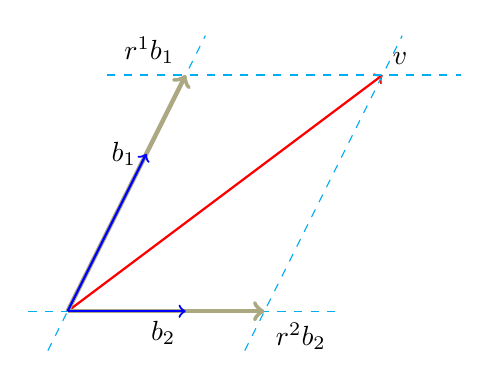
\begin{tikzpicture}
      \draw [->, thick, red] (0, 0) -- (4, 3) node [above right, black] {$\rvec{v}$};

      \draw [dashed, magenta, cyan] (-0.25, -0.5) -- (1.75, 3.5);
      \draw [dashed, magenta, cyan] (2.25, -0.5) -- (4.25, 3.5);

      \draw [dashed, magenta, cyan] (-0.5, 0) -- (3.5, 0);
      \draw [dashed, magenta, cyan] (0.5, 3) -- (5, 3);

      \draw [->, ultra thick, yellow!25!gray]
      (0, 0) -- (1.5, 3) node [above left, black] {$r^1\rvec{b}_1$};
      \draw [->, ultra thick, yellow!25!gray]
      (0, 0) -- (2.5, 0) node [below right, black] {$r^2\rvec{b}_2$};

      \draw [->, thick, blue] (0, 0) -- (1, 2)
      node [left, black] {$\rvec{b}_1$};
      \draw [->, thick, blue] (0, 0) -- (1.5, 0)
      node [below left, black] {$\rvec{b}_2$};
    \end{tikzpicture}

    \caption{Kontravariáns koordináták}
  \end{figure}
\end{minipage} \hfill
\begin{minipage}[c]{.45\textwidth}
  \begin{figure}[H]
    \centering
    \begin{tikzpicture}
      \tkzDefPoints{0/0/O/, 4/2/E, 1/2/A, 1.5/0/B}
      \tkzDefPointBy[projection = onto O--A](E)  \tkzGetPoint{P}
      \tkzDefPointBy[projection = onto O--B](E)  \tkzGetPoint{Q}

      \tkzDrawLines[add=.15 and .15, dashed, cyan](O,P E,P O,Q E,Q)

      % \tkzDrawSegment[color=red, thick, ->](O,E)
      %
      % TBD nicer
      %

      \draw [->, thick, red] (O) -- (E)
      node [above right, black] {$\rvec{v}$};

      \draw [->, ultra thick, yellow!25!gray]
      (O) -- (P) node [left, black] {$r_1\rvec{b}_1$};
      \draw [->, ultra thick, yellow!25!gray]
      (O) -- (Q) node [below right, black] {$r_2\rvec{b}_2$};

      \draw [->, thick, blue] (O) -- (A)
      node [left, black] {$\rvec{b}_1$};
      \draw [->, thick, blue] (O) -- (B)
      node [below left, black] {$\rvec{b}_2$};

      \tkzMarkRightAngles[german, size=.4](O,P,E E,Q,O)
    \end{tikzpicture}

    \caption{Kovariáns koordináták}
  \end{figure}
\end{minipage} \hfill

\vspace*{1.5em}
$\rvec{v} = r^1 \rvec{b}_1 + r^2 \rvec{b}_2$, ahol
$(r^1 ; \; r^2)$ a $\rvec{v}$ vektor kontravariáns koordinátái
a $\left\{ \rvec{b}_1 ; \; \rvec{b}_2 \right\}$ bázisban.

\vspace*{.5em}
$r_1$ és $r_2$ pedig $\rvec{v}$ kovariáns koordinátái,
melyek a következőképpen számíthatóak:
\begin{equation*}
  r_i \, \rvec{b}_i = \frac{
    \scalar{\rvec{v}}{\rvec{b}_i}
  }{\norma{\rvec{b}_i}} \cdot \frac{
    \rvec{b}_i
  }{\norma{\rvec{b}_i}}
  = \underbrace{\rected{$\displaystyle\frac{
          \scalar{\rvec{v}}{\rvec{b}_i}
        }{\scalar{\rvec{b}_i}{\rvec{b}_i}}$}{yellow}}_{r_i}
  \cdot \rvec{b}_i
\end{equation*}


\allit{0}{.33}

Kovariáns és kontravariáns koordináták ortonormált
$\left\{ \uvec{e}_1 ; \; \uvec{e}_2 ; \; \dots \; \uvec{e}_n \right\}$
bázisban megegyeznek.

\biz{1}{0}

\begin{equation*}
  \rvec{v} = \sum_{j=1}^n r^j \uvec{e}_j
\end{equation*}
\begin{equation*}
  r^j = \dfrac{
    \scalar{\rvec{v}}{\uvec{e}_j}
  }{
    \scalar{\uvec{e}_j}{\uvec{e}_j}
  } = \; \scalar{\rvec{v}}{\uvec{e}_j}
\end{equation*}
\begin{equation*}
  r_j = \; \scalar{
    \sum_{i=1}^n r^i \, \uvec{e}_i
  }{\uvec{e}_j} \; = \sum_{i=1}^n r^i \underbrace{
    \scalar{\uvec{e}_i}{\uvec{e}_j}
  }_{\displaystyle\delta_{ij}} \; = r^j
\end{equation*}

%-------------------------------------------------------------------------------
%-------------------------------- Subsection 1.3 -------------------------------
%-------------------------------------------------------------------------------
\subsection{Lineáris leképezések}

\defi{0}{.33}{Lineáris leképezés adjungáltja}

$! \; (V; \, \scalar{}{})$ Euklideszi tér,
$\varphi: V \rightarrow V$ lineáris leképezés.
A $\varphi^{*} : V \rightarrow V$ lineáris leképezést
a $\varphi$ leképezés adjungáltjának hívjuk, ha
$\scalar{\varphi(\rvec{v}_1)}{\rvec{v}_2}
  \; = \; \scalar{\rvec{v}_1}{\varphi(\rvec{v}_2)}$
$\forall \; \rvec{v}_1 ;\; \rvec{v}_2 \in V$.

\allit{1}{.33}
$\left( \varphi^{*} \right)^{*} = \varphi$
\hspace{2mm} – \hspace{2mm} (Idempotencia)

\biz{1}{.33}
$\scalar{\left( \varphi^{*} \right)^{*}(\rvec{v}_1)}{\rvec{v}_2}
  \; = \; \scalar{\rvec{v}_1}{\varphi^{*}(\rvec{v}_2)}
  \; = \; \scalar{\varphi(\rvec{v}_1)}{\rvec{v}_2}$
\end{document}